\documentclass[english]{tudscrreprt}
\usepackage[T1]{fontenc}
%\usepackage[ngerman=ngerman-x-latest]{hyphsubst}
\usepackage{babel}
\usepackage{isodate}
\usepackage{tudscrsupervisor}
\usepackage{enumitem}\setlist{noitemsep}
\usepackage{siunitx}
\usepackage{tabto}

\begin{document}
\faculty{Faculty of Electrical and Computer Engineering}
\institute{Institute of Electrical Power Engineering}\chair{Chair of Electromagnetic Theory and Compatibility}
\title{%
Large GTEM-Cell
}\date{\today}
\contactperson{%
Prof. Hans Georg Krauthäuser\emailaddress{tetemv@tu-dresden.de}
\office{Görges-Bau, Room 223}\telephone{+49 351 463-33357}
%\and%
%Mac Moneysac\emailaddress{mac.moneysac@tu-dresden.de}
%\office{Dingens-Bau, Zimmer~15}\telephone{+49 351 463-54321}
}
\noticeform[headline=Laboratory Description,pagestyle=empty]{%
  \renewcommand{\focusname}{Parameter}
  \renewcommand{\contactpersonname}{Contact Person}
 GTEM cells are alternative test environments to free fields and anechoic chambers.

The main field of application for GTEM cells is EMC emission and immunity measurements for smaller test objects. Compared to measurements with antennas, GTEM cells can also be used to carry out measurements at relatively low frequencies on a laboratory scale. In addition, GTEM cells are ideal for measurements in the time domain (e.g. also for transfer functions and shield attenuation measurements).
\begin{center}
  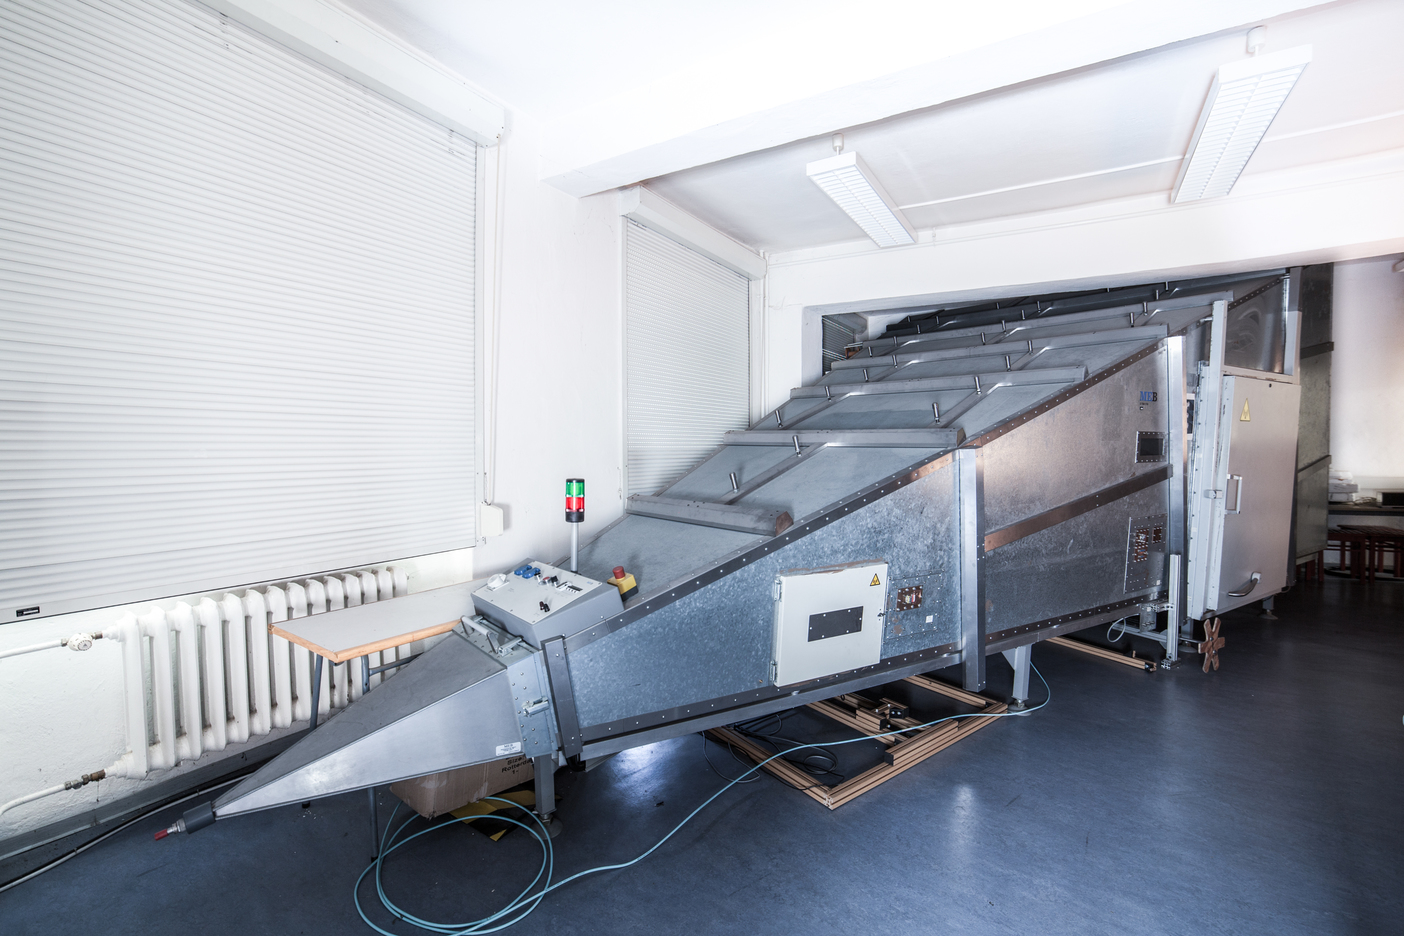
\includegraphics[width=.65\linewidth]{gtem_cell_aussen_hell_klein}
\renewcommand*{\figureformat}{Photo}
\captionof{figure}{View of the Large GTEM-Cell.}
\end{center}
}{%
\item Frequency range:\tabto{.3\linewidth} \qtyrange{0}{18}{\giga\hertz}
\item Field Strength: \tabto{.3\linewidth} $\le$ \qty{10}{\volt\per\metre}
\item EUT-Volume ($l \times w \times h$): \tabto{.3\linewidth} $\qty{1}{\metre} \times \qty{1}{\metre} \times \qty{0.75}{\metre}$
\item Available Power: \tabto{.3\linewidth} \qtyrange{1}{4200}{\mega\hertz}: \qty{30}{\watt}
\item Main Standards:
  \begin{itemize}
  \item IEC~61000-4-20, EN~61000-4-20, DIN~EN~61000-4-20
    \end{itemize}
}
\end{document}